%!TEX root = ../main.tex
%
%
\begin{figure}[t!]
\centering
\footnotesize
\begin{tabular}{@{}c@{\;}c@{\;}}
%
%=====================
%
%\rotatebox{90}{\quad\quad Multi-jitter} & 
\begin{tikzpicture}
  \node[anchor=south west,inner sep=0] (image) at (0,0)
  {
    \pdfliteral{ 1 w}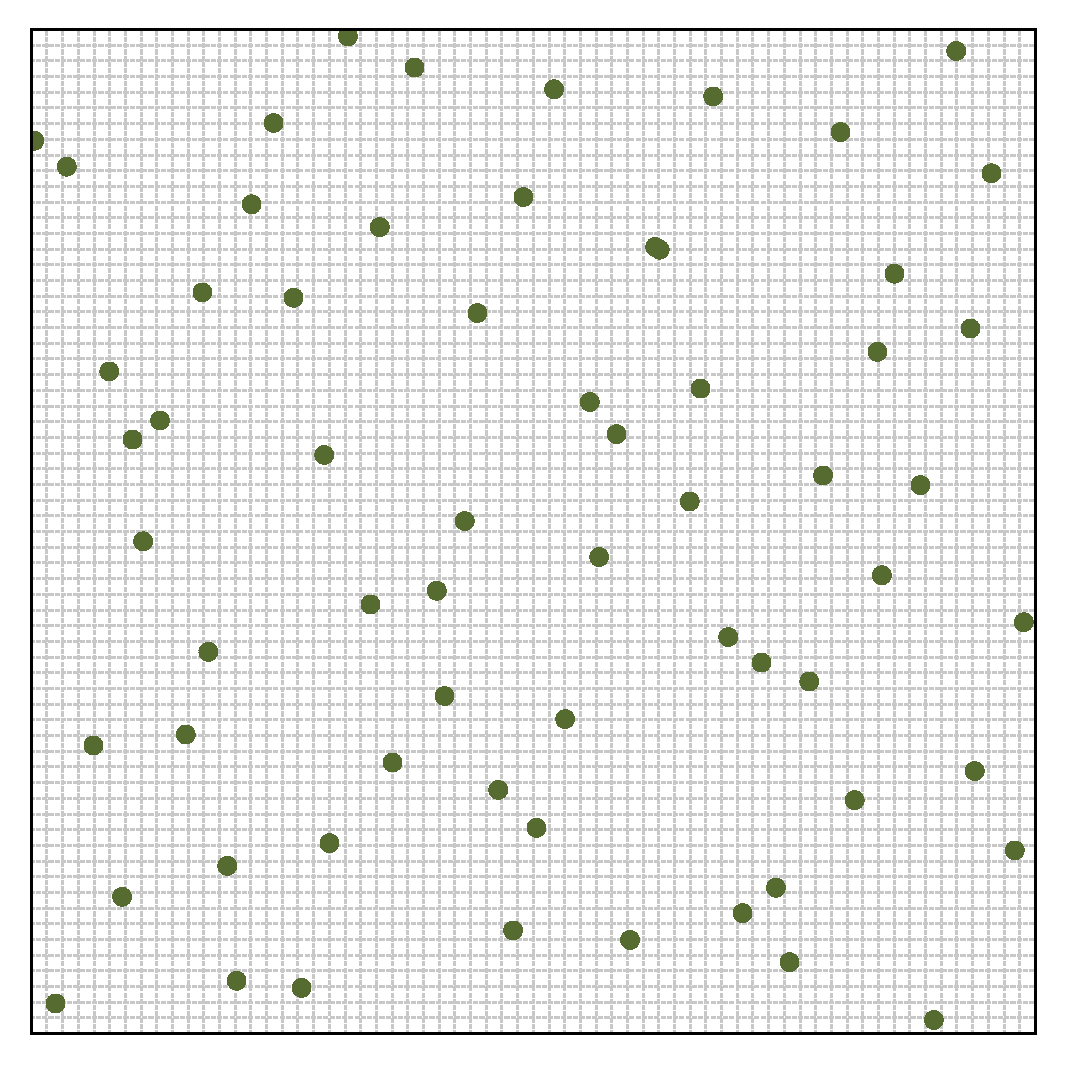
\includegraphics[width=0.4\columnwidth,page=1]{pointset-gridvisualize/points-multijitter-n64.pdf}
  };

%  \begin{scope}[x={(image.south east)},y={(image.north west)}]
%  \draw[black,thick] (0,0) rectangle (1,1);
%  \end{scope}
\end{tikzpicture} 
&
\begin{tikzpicture}
  \node[anchor=south west,inner sep=0] (image) at (0,0)
  {
    \pdfliteral{ 1 w}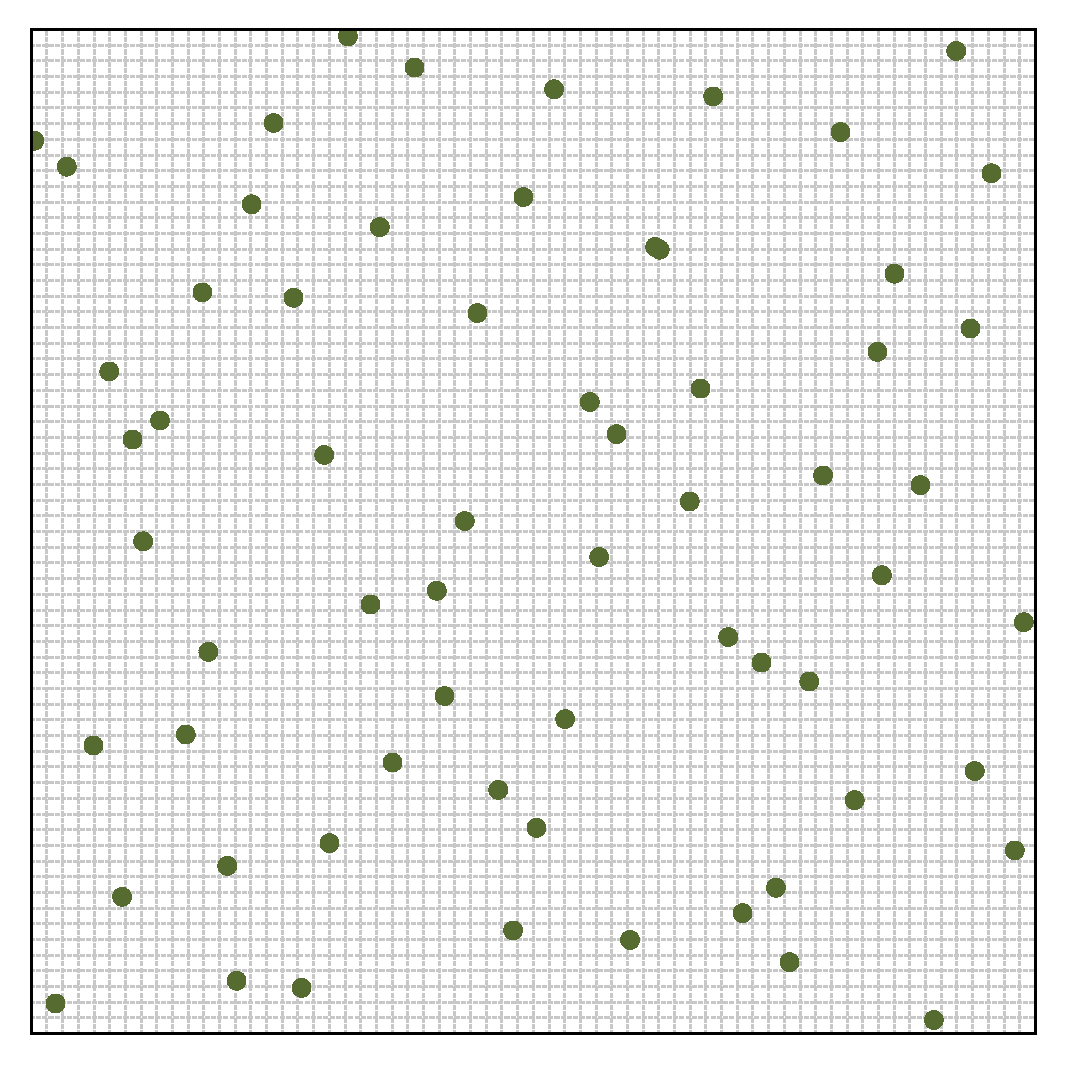
\includegraphics[width=0.4\columnwidth,page=1]{pointset-gridvisualize/points-multijitter-n64.pdf}
  };

%  \begin{scope}[x={(image.south east)},y={(image.north west)}]
%  \draw[black,thick] (0.01,0.01) rectangle (0.99,0.99);
%  \end{scope}
\end{tikzpicture}\\
\end{tabular}
%
\caption{\label{fig:points-powspec-radialmean}%
Illustration of some well known sampling patterns in 2D with the corresponding Fourier expected power spectra and the corresponding radial mean of their expected power spectra.}
\end{figure}